\documentclass[a4paper, 12pt]{article}
\usepackage[utf8]{inputenc}
\usepackage[slovak]{babel}
\usepackage{graphicx}
\usepackage{amsmath,amssymb,amsfonts}

\newenvironment{task}{}{}
\newenvironment{solution}{\noindent\textbf{Riešenie:}}{}

\begin{document}


\section*{B36B6A}
\begin{task}
    Nájdite prenosovú funkciu 
    \begin{equation*}
        F(s)=\dfrac{Y(s)}{W(s)}
    \end{equation*}
     pre systém opísaný blokovou schémou: 

    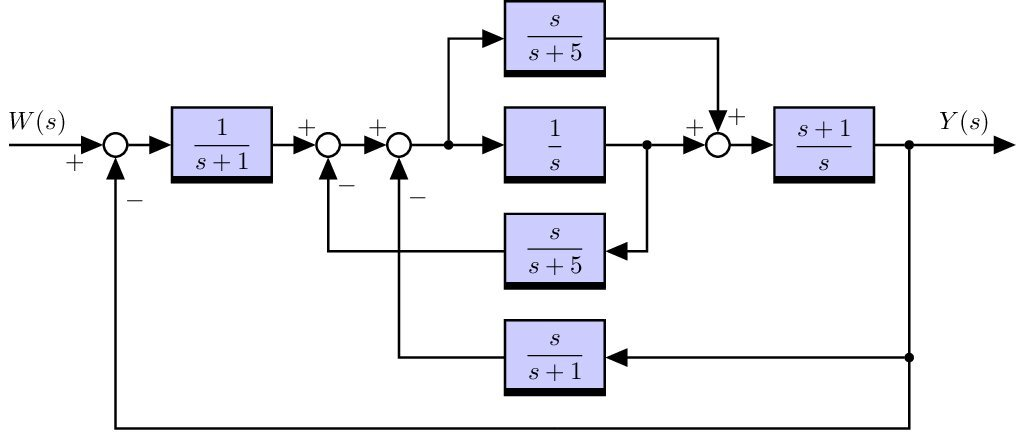
\includegraphics{blokovka02_00002.jpg} 
\end{task} 

\begin{solution}
    \begin{equation*}
        \dfrac{s^2+s+5}{2s^3+8s^2+6s+5}
    \end{equation*}
\end{solution}

\section*{BB9B40}
\begin{task}
    Nájdite prenosovú funkciu 
    \begin{equation*}
        F(s)=\dfrac{Y(s)}{W(s)}
    \end{equation*}
     pre systém opísaný blokovou schémou: 

    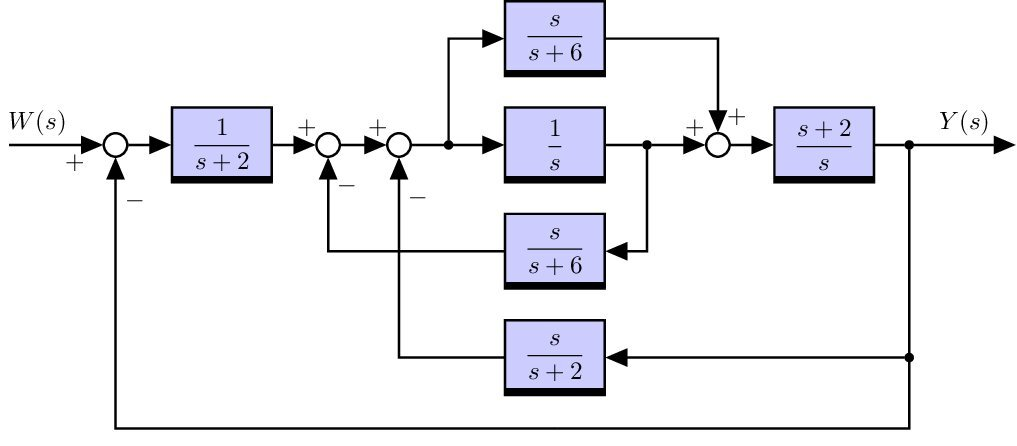
\includegraphics{blokovka02_00003.jpg} 
\end{task} 

\begin{solution}
    \begin{equation*}
        \dfrac{s^2+s+6}{2s^3+9s^2+7s+6}
    \end{equation*}
\end{solution}
%\newpage
\section*{B35B6C}
\begin{task}
    Nájdite prenosovú funkciu 
    \begin{equation*}
        F(s)=\dfrac{Y(s)}{W(s)}
    \end{equation*}
     pre systém opísaný blokovou schémou: 

    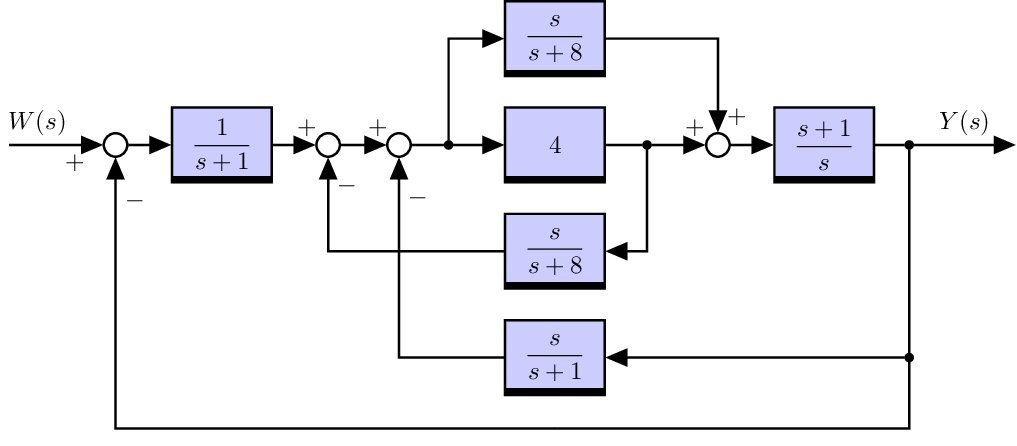
\includegraphics{blokovka02_00004.jpg} 
\end{task} 

\begin{solution}
    \begin{equation*}
        \dfrac{5s+32}{10s^2+45s+32}
    \end{equation*}
\end{solution}


\end{document}
